%\subsection{Trajectory Length}
%
%\subsection{Cloud Techniques: Elastic Search}
%
%What if we re-provision resources in response to events outside the
%application's control, such as a slow Lustre.
%
%\subsection{Future work}
%
%How Much: cache policy from past, regime detection, Belady's Min

\section{Cache Management Using Storage System Architecture Knowledge}
\label{sec:arch-specific}

Using the Mantle policy engine, we test a variety of cache management 
algorithms on the worker using the keyspace analysis in
Section~\S\ref{sec:parsplice-keyspace-analysis}.  Our evaluation uses the total
``trajectory length" as the goodness metric. This value is the duration of the
overall trajectory produced by ParSplice. At ideal efficiency, the trajectory
length should increase with the square root of the wall-clock time, since the
wall-clock cost of time-stepping the system by one simulation time unit
increases in proportion of the total number of atoms.  The policy should avoid
reducing the trajectory length and be fast enough to run as often as we want to
detect key access patterns.  First we size the cache according to our system
specific knowledge, {\it i.e.} the hardware and software of the storage
hierarchy.

% technical details
We implement a basic LRU cache using a ``when" policy of:

\begin{figure}[h]
\footnotesize
\begin{minted}{lua}
server[whoami]['cachesize']>n
\end{minted}
\end{figure}

and a ``how much" policy of:

\begin{figure}[h]
\footnotesize
\begin{minted}{lua}
servers[whoami]['cachesize']-n
\end{minted}
\end{figure}

The results for different cache sizes for a growth rate of \(\Delta_1\) over a
2.5 hour run across 256 workers is shown in
Figure~\ref{fig:methodology-tradeoff}.  ``Baseline" is the performance of
unmodified ParSplice  measured in trajectory duration (\(y1\) axis) and
utilization is measured with memory footprint of just the cache (\(y2\) axis).
The middle graph labeled ``Fixed Cache Size" shares the \(y\) axes and shows
the trade-off of using a basic LRU-style cache of different sizes, where the
penalty for a cache miss is retrieving the data from the persistent database.
The error bars are the standard deviation of 3 runs.  Although the keyspace
grows to 150K, a 100K key cache achieves 99\% of the performance. Decreasing
the cache degrades performance and predictability.

%\begin{figure}[h] \footnotesize \begin{minted}{lua}
%server[whoami]['cachesize'] > n \end{minted} \end{figure}

%and ``how much":
%\begin{figure}[h]
%\footnotesize
%\begin{minted}{lua}
%servers[whoami]['cachesize'] - n
%\end{minted}
%\end{figure}


\begin{figure}[t]
\noindent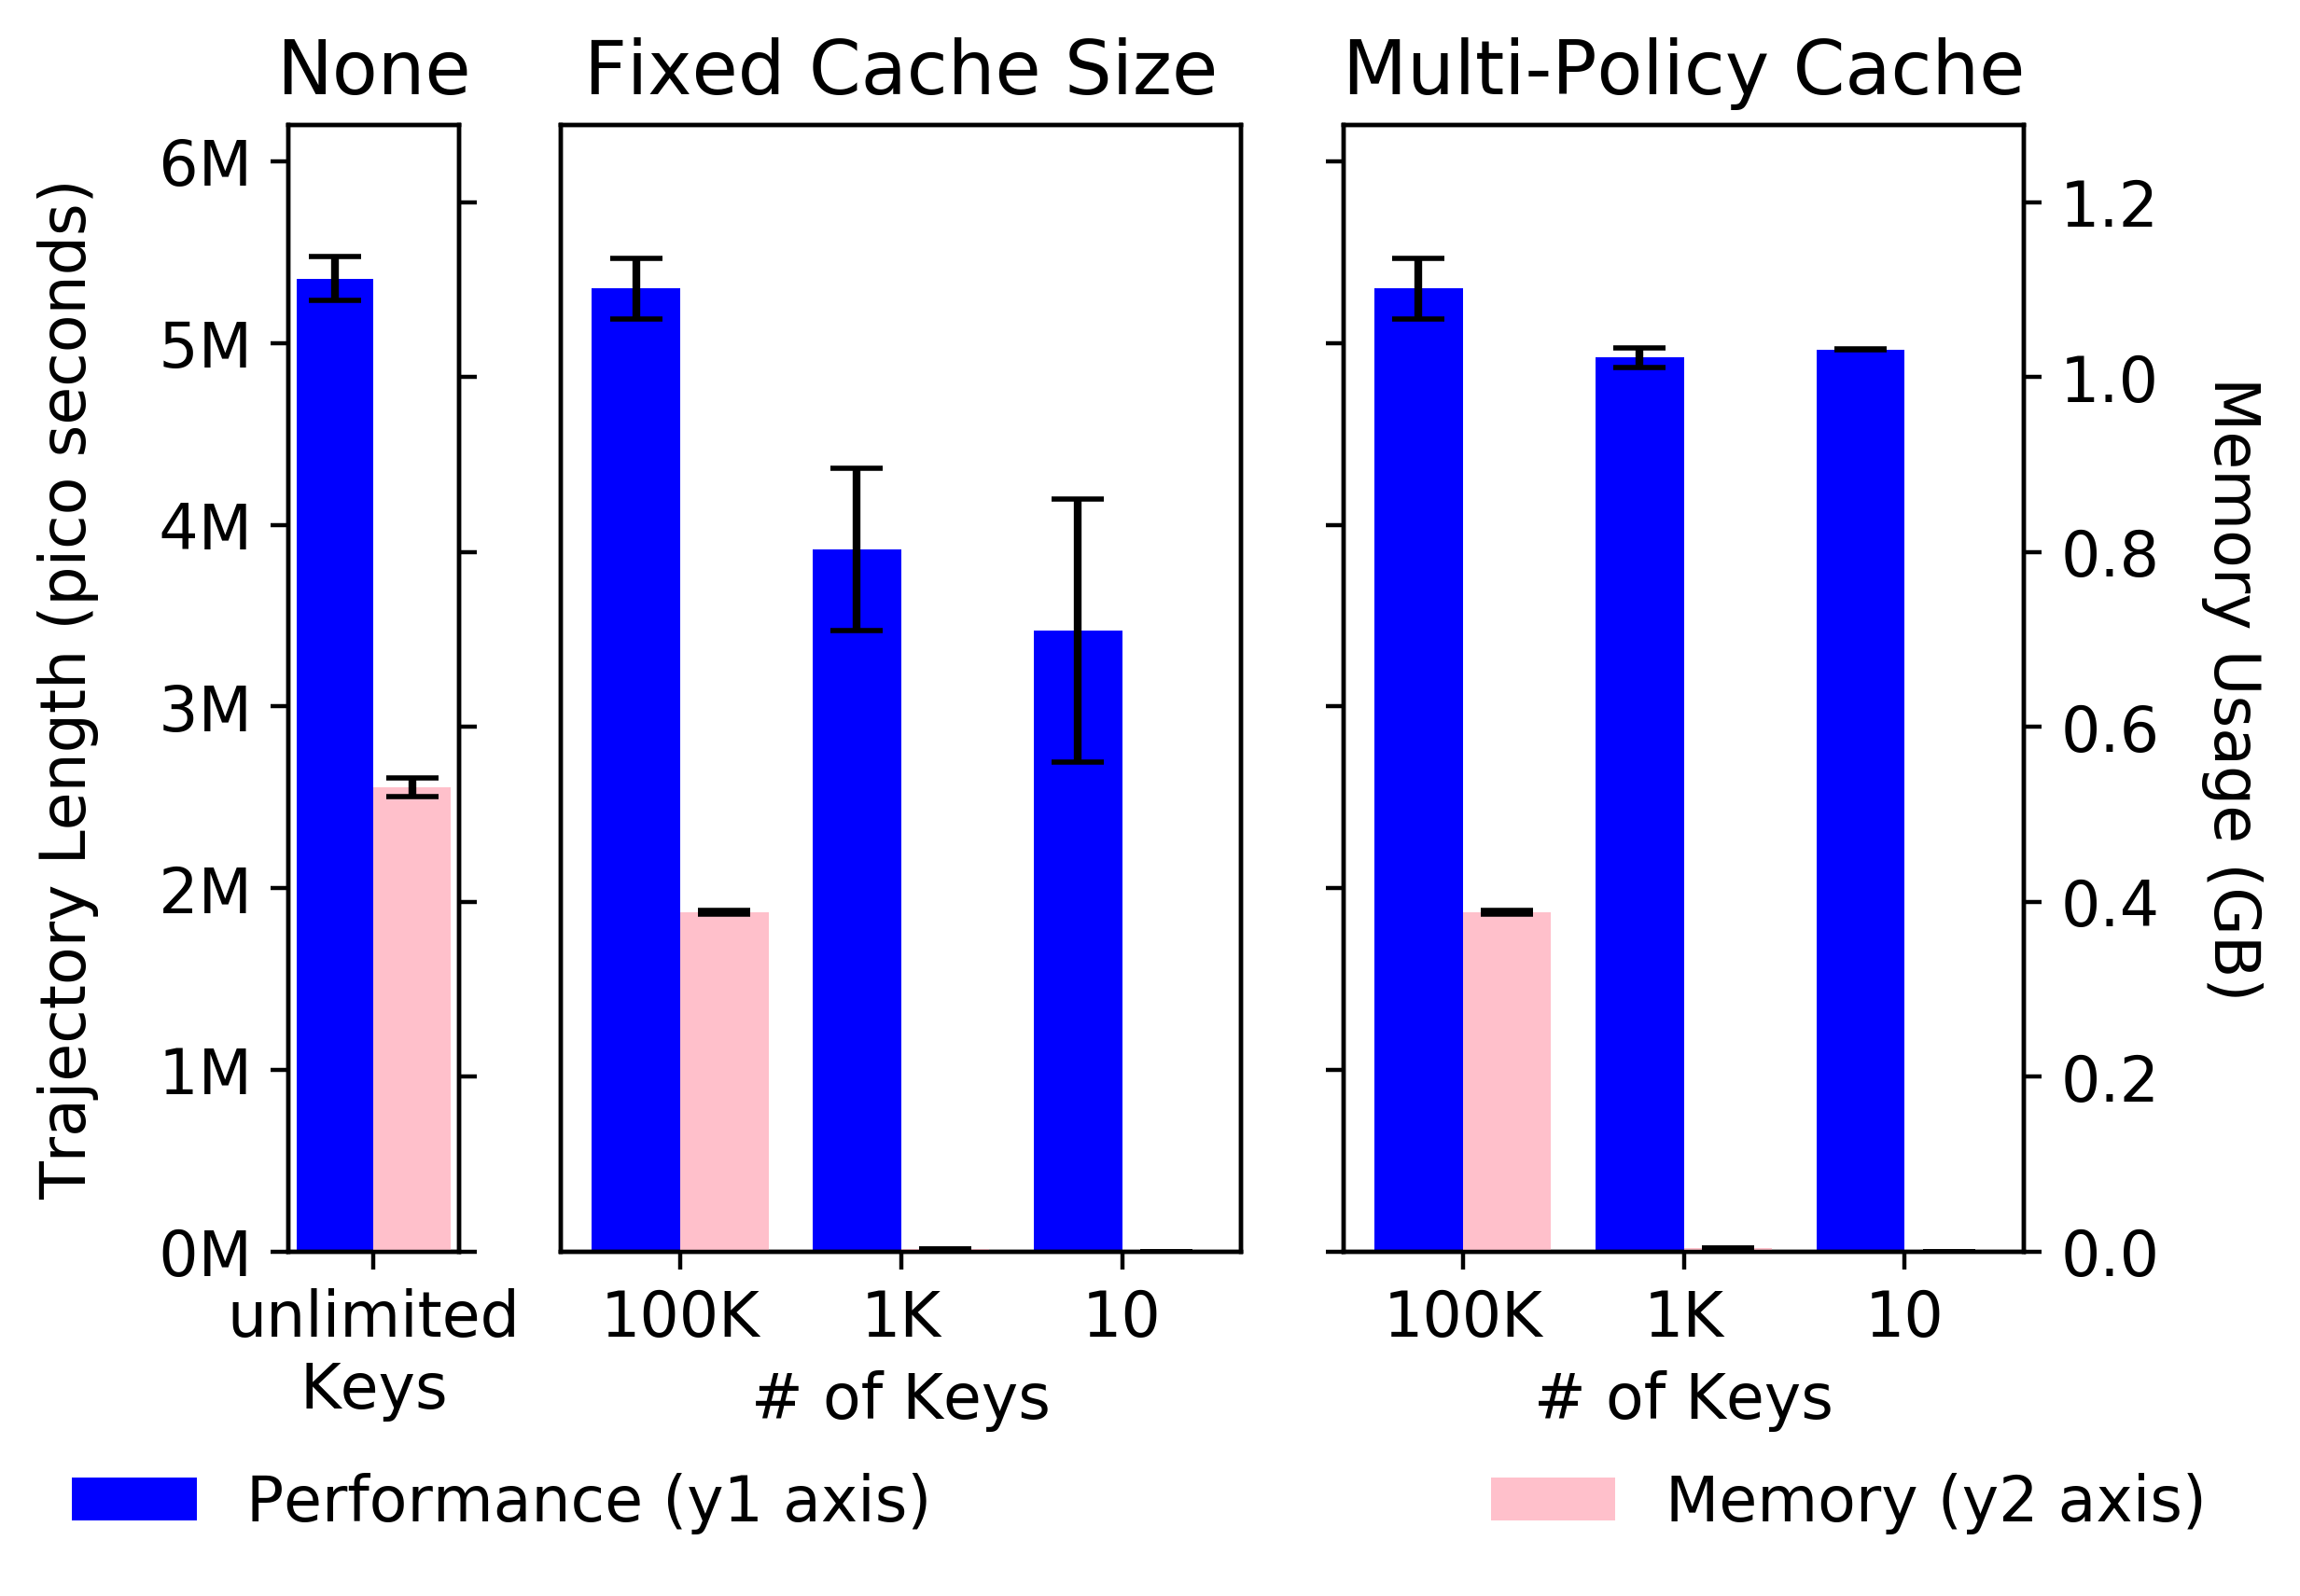
\includegraphics[width=0.5\textwidth]{./chapters/controlplane/parsplice/figures/methodology-tradeoff.png}\\
\caption{Policy performance/utilization shows the trade-offs of different sized
caches (\(x\) axis).  ``None" is ParSplice unmodified, ``Fixed Sized Cache"
evicts keys using LRU, and ``Multi-Policy Cache" switches to fixed sized cache
after absorbing the workload's initial burstiness. This parameter sweep
identifies the ``Multi-Policy Cache" of 1K keys as the best solution but this
only works for this system setup and initial configurations.
 \label{fig:methodology-tradeoff}}
\end{figure}

\begin{figure}[t]
        \centering
        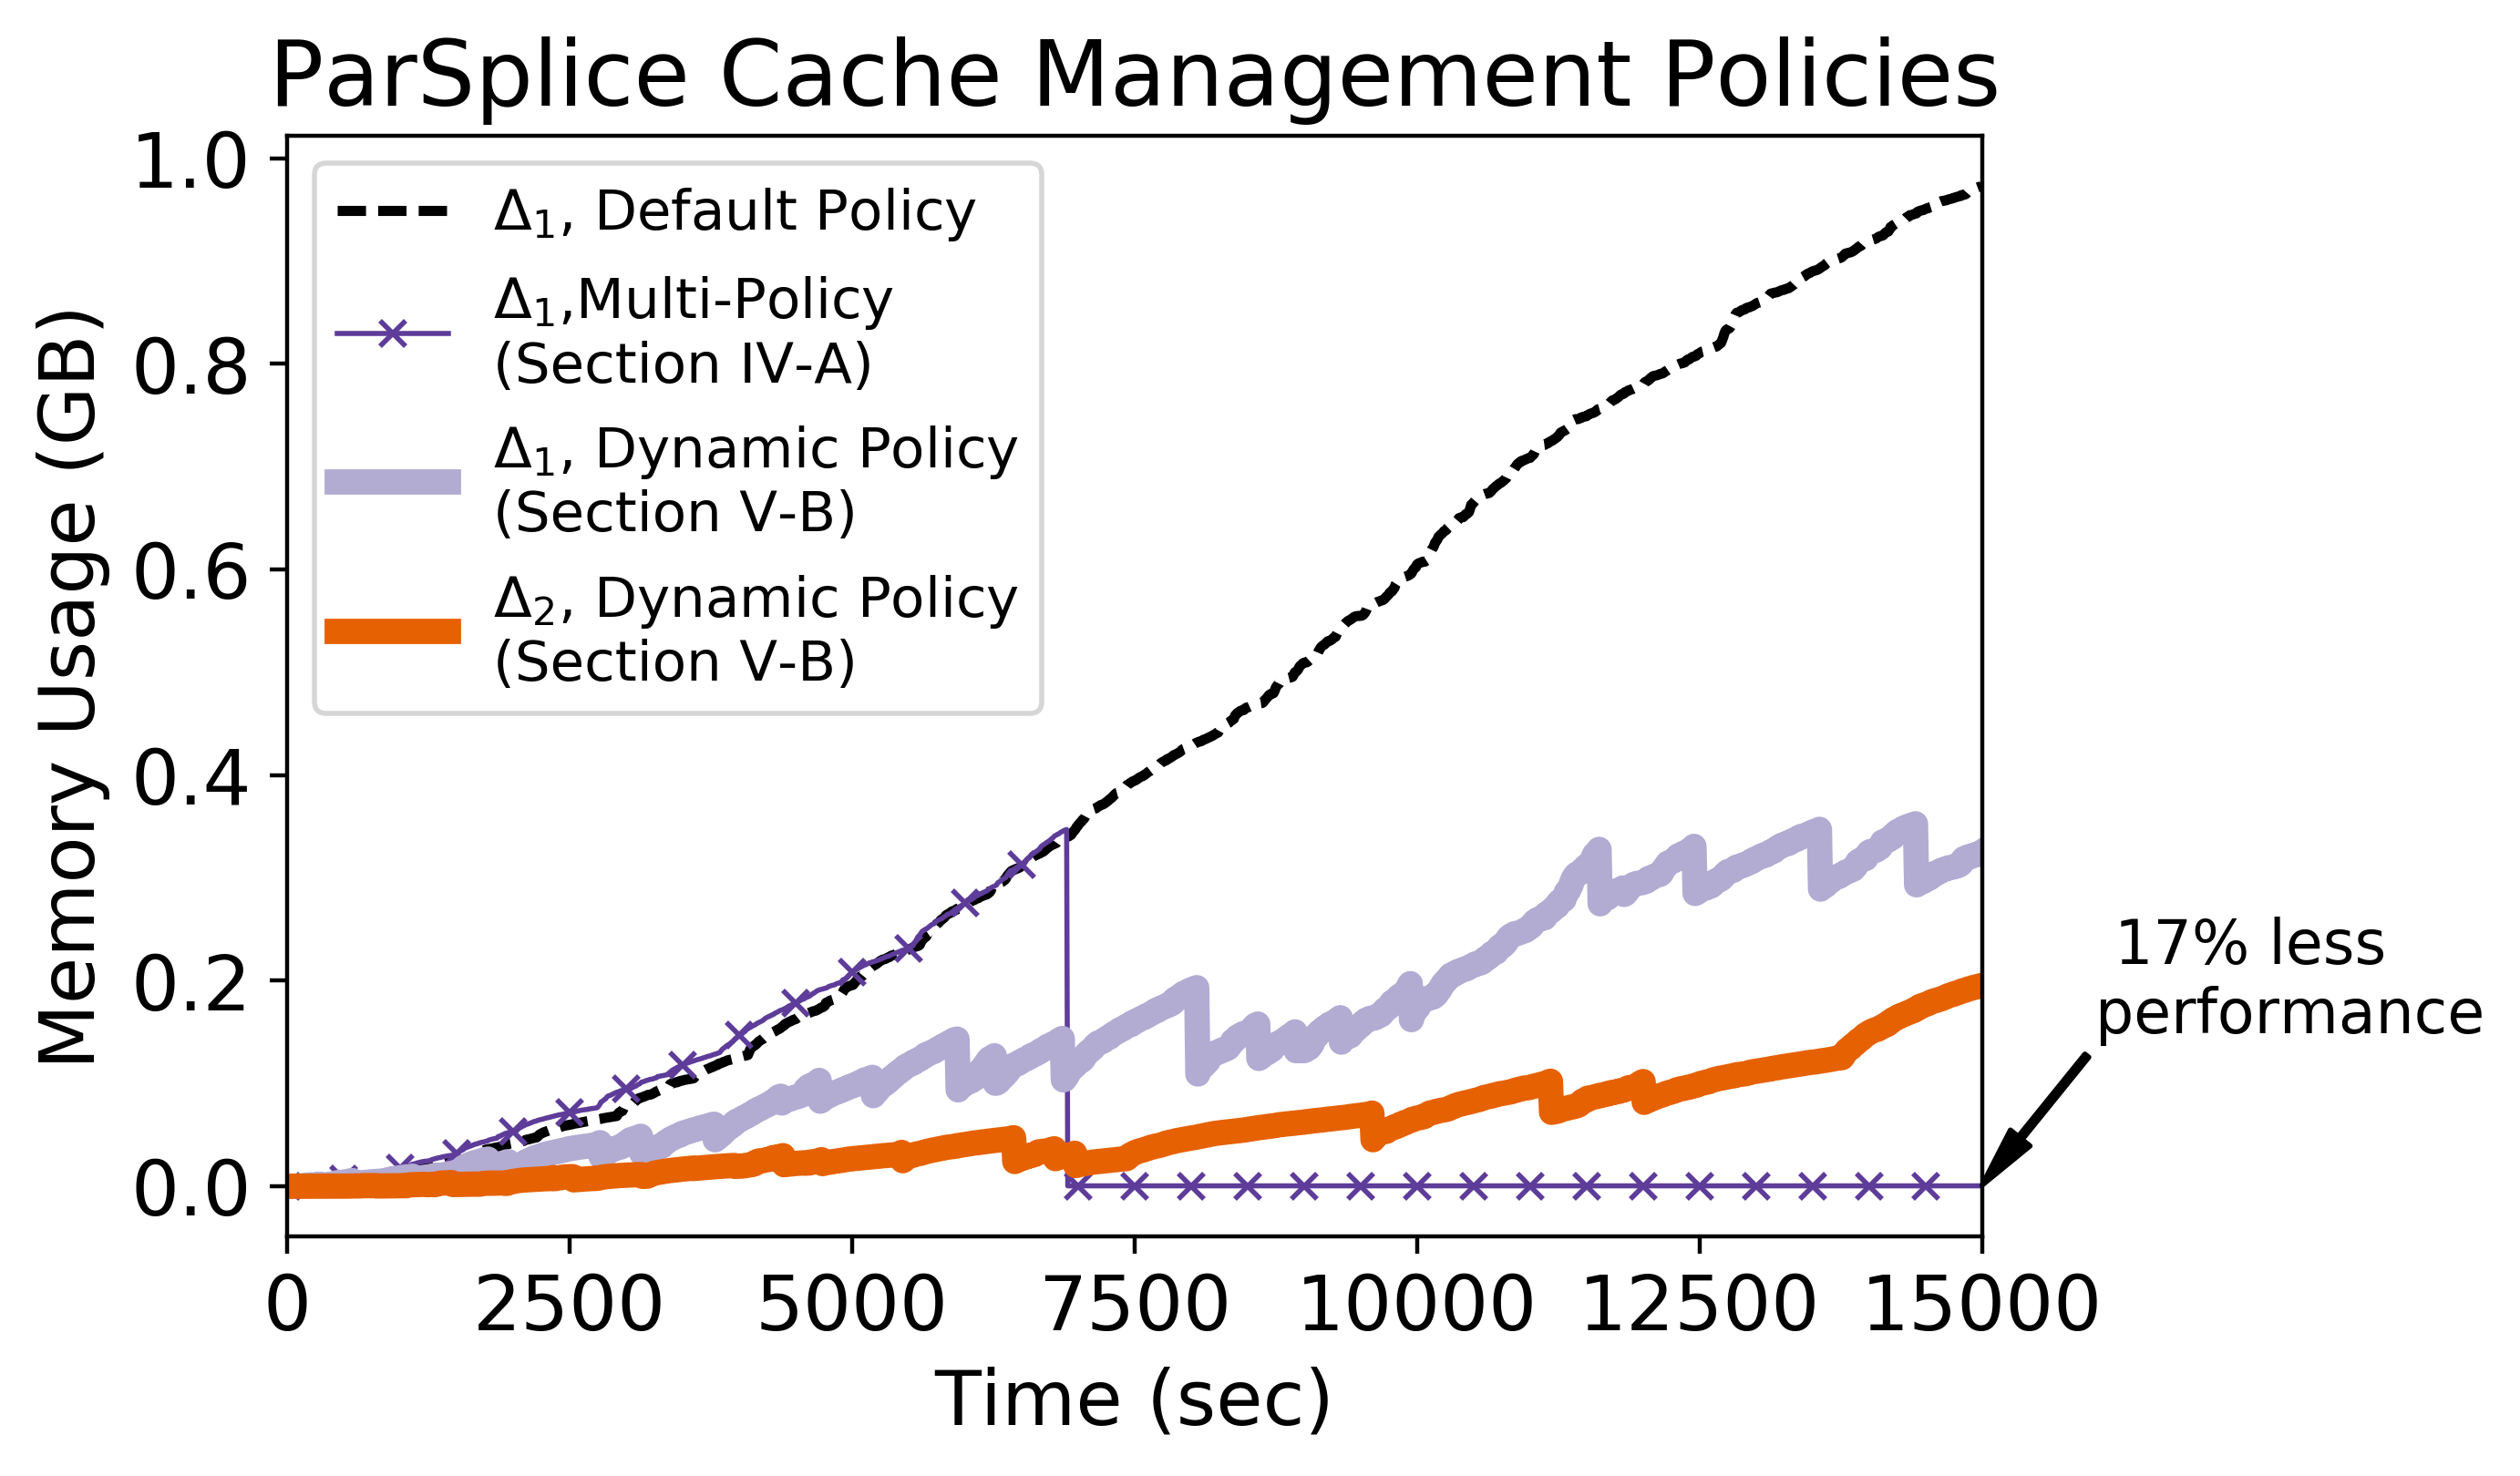
\includegraphics[width=0.5\textwidth]{./chapters/controlplane/parsplice/figures/memory-vs-time.png}\\
	\caption{Memory utilization for ``No Cache Management" (unlimited cache
growth), ``Multi-Policy" (absorbs initial burstiness of workload), and
``Dynamic Policy" (sizes cache according to key access patterns). The dynamic
policies saves the most memory without sacrificing performance.
\label{fig:memory-vs-time}}
\end{figure}%
 


%
%\footnotesize \centering \begin{minted}[xleftmargin=3em,linenos]{lua} function
%when() if server[whoami]['cachesize'] > n then return true end return false
%end
%
%function howmuch() if servers[whoami]['cachesize'] > n return
%servers[whoami]['cachesize'] - n end return 0 end \end{minted} \caption{Policy
%that implements a basic LRU cache. The performance and memory utilization for
%different values of \(n\) are graphed in
%Figure~\ref{fig:methodology-tradeoff}.  \label{src:lru}} \end{figure}

% why is the performance lower for smaller caches?
But the top graph in Figure~\ref{fig:motivation-regimes} suggests that a
smaller cache size should suffice, as only 100 keys seem to be active at any
one time.  It turns out that the unique keys plotted in
Figure~\ref{fig:motivation-regimes} are per second and are not representative
of the actual active keyspace; the number of active keys is larger than 100, as
some keys may be accessed at time \(t_0\), not in \(t_1\), and then again in
\(t_2\). Because the cache is too small, reads and writes fall through to the
rest of the storage hierarchy and the excessive traffic triggers a LevelDB
compaction on the persistent database.  To avoid these compactions, which
temporarily block operations, we design a multi-policy cache that switches
between:

\begin{itemize}
  \item unlimited growth policy: cache increases on every write
  \item \(n\) key limit policy: cache constrained to \(n\) keys
\end{itemize}

% results: same level of performance can be achieved 
The key observation is that small caches incur too much load on the persistent
database at the beginning of the run but should suffice after the initial read
flash crowd passes because the keyspace is far less active.  We program Mantle
to trigger the policy switch at 100K keys to absorb the flash crowd at the
beginning of the run. Once triggered, keys are evicted to bring the size of the
cache down to the threshold.  The actual policy is shown and described in more
detail in Section~\S\ref{sec:scope} in Figure~\ref{src:lru-dyn}.  The plot on
the right side of Figure~\ref{fig:methodology-tradeoff} shows the
performance/utilization trade-off of the multi-policy cache, where the cache
sizes for the \(n\) key limit policy are along the \(x\) axis.  The performance
and memory utilization for a 100K key cache size is the same as the 100K bar in
the ``Fixed Cache Size" graph in Figure~\ref{fig:methodology-tradeoff} but the
rest reduce the size of the keyspace after the read flash crowd.  We see the
worst performance when the policy switches to the 10 key limit policy, which
achieves 94\% of the performance while only using 40KB of memory. 

% caveats: it is calculating 90% of the trajectory, memory value reported is final
\subsubsection*{Caveats}

The results in Figure~\ref{fig:methodology-tradeoff} are slightly deceiving for
two reasons: (1) segments take longer to generate later in the run and (2) the
memory footprint is the value at the end of 2.5 hours.  For (1), the trajectory
length vs.  wall-clock time curves down over time; as the nanoparticle grows it
takes longer to generate segments so by the time we reach 2 hours, over 90\% of
the trajectory is already generated.  For (2), the memory footprint rises until
it reaches the 100K key switch threshold at 0.4GB and then reduces to the final
value after switching policies. The memory usage over time for this policy is
shown by the ``\(\Delta_1\), Multi-Policy" curve in
Figure~\ref{fig:memory-vs-time} but in Figure~\ref{fig:methodology-tradeoff} we
plot the final value.  Despite these caveats, the result is still valid: we
found a multi-policy cache management strategy that absorbs the cost of a high
read throughput on a small keyspace and reduces the memory pressure for a 2.5
hour run.  To improve the policy even more, we need a way to identify what
thresholds to use for different system setups ({\it e.g.}, different ParSplice
parameters, number of worker tasks, and job lengths).  

\section{Cache Management Using Application-Specific Knowledge}
\label{sec:dom-specific}

\begin{figure*}[t!]
    \begin{subfigure}[t]{0.48\textwidth}
        \centering
	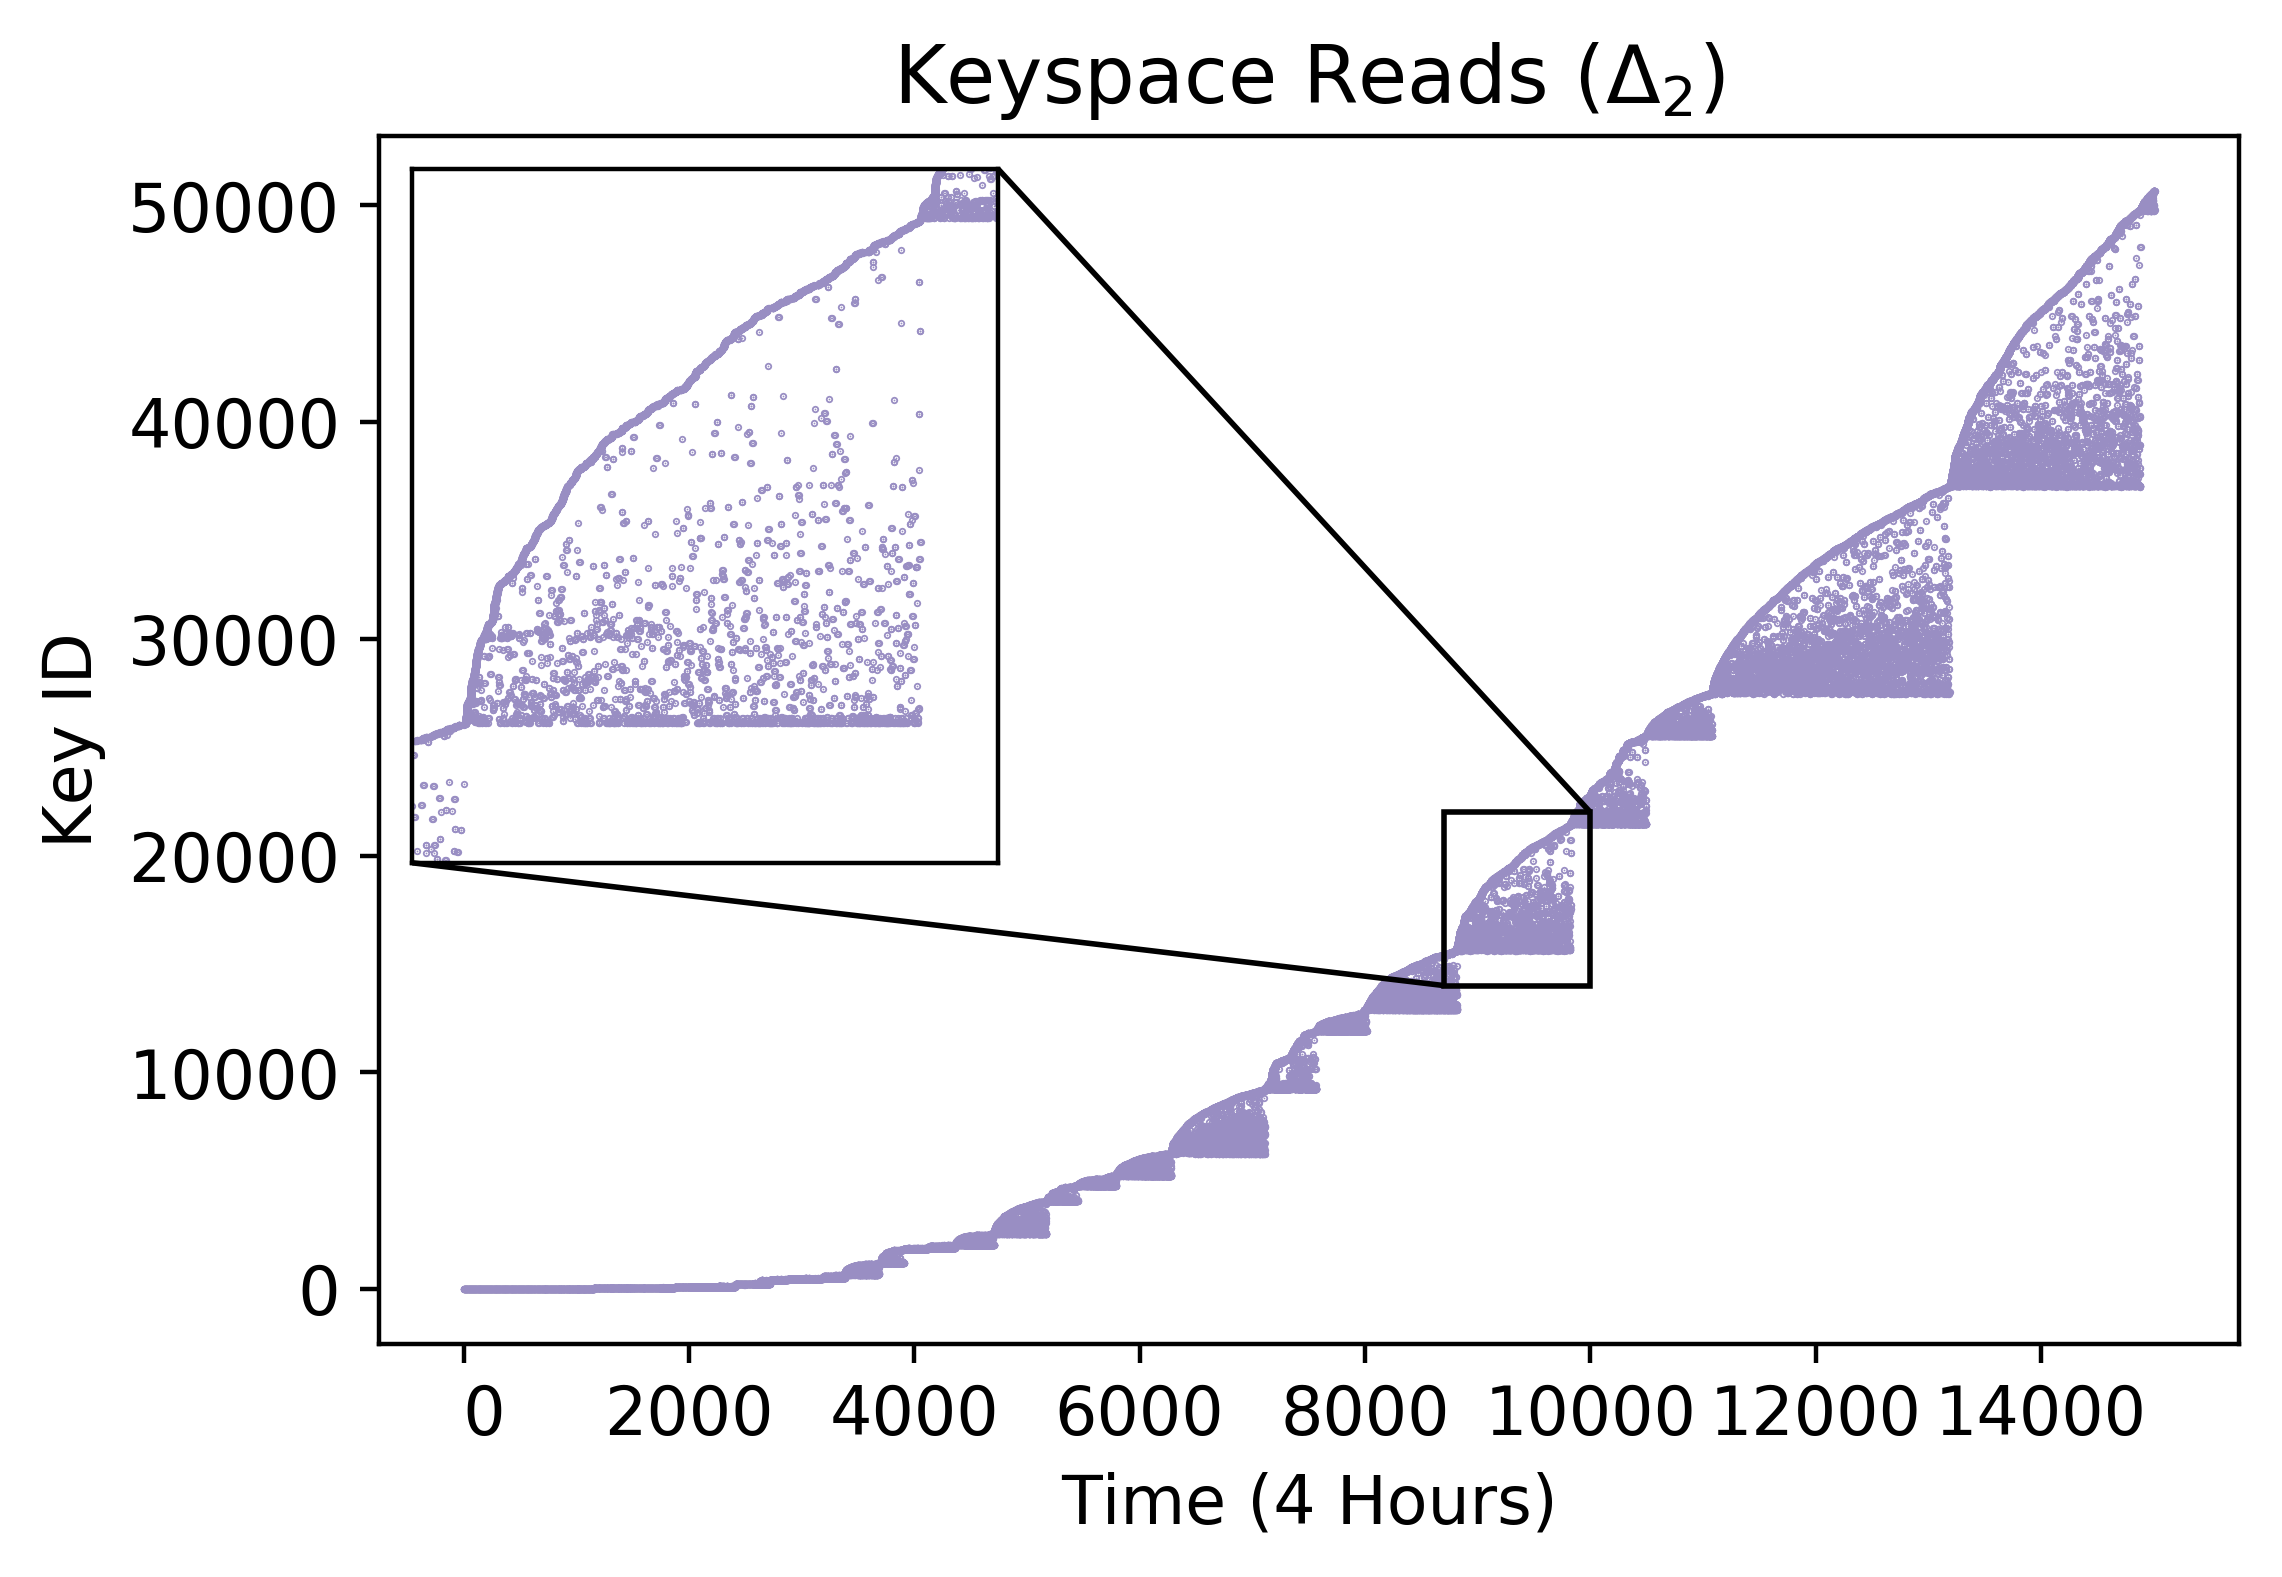
\includegraphics[width=1\textwidth]{./chapters/controlplane/parsplice/figures/keyspace-zoomed.png}\\

\caption{Key activity for a 4 hour run shows groups of accesses to the same
subset of keys. Detecting these access patterns leads to a more accurate cache
management strategy, which is discussed in Section~\S\ref{sec:regime-detection}
and the results are in Figure~\ref{fig:dscache-vs-none}.
\label{fig:keyspace-zoomed}}
    \end{subfigure}%
    ~ 
    \begin{subfigure}[t]{0.48\textwidth}
        \centering
        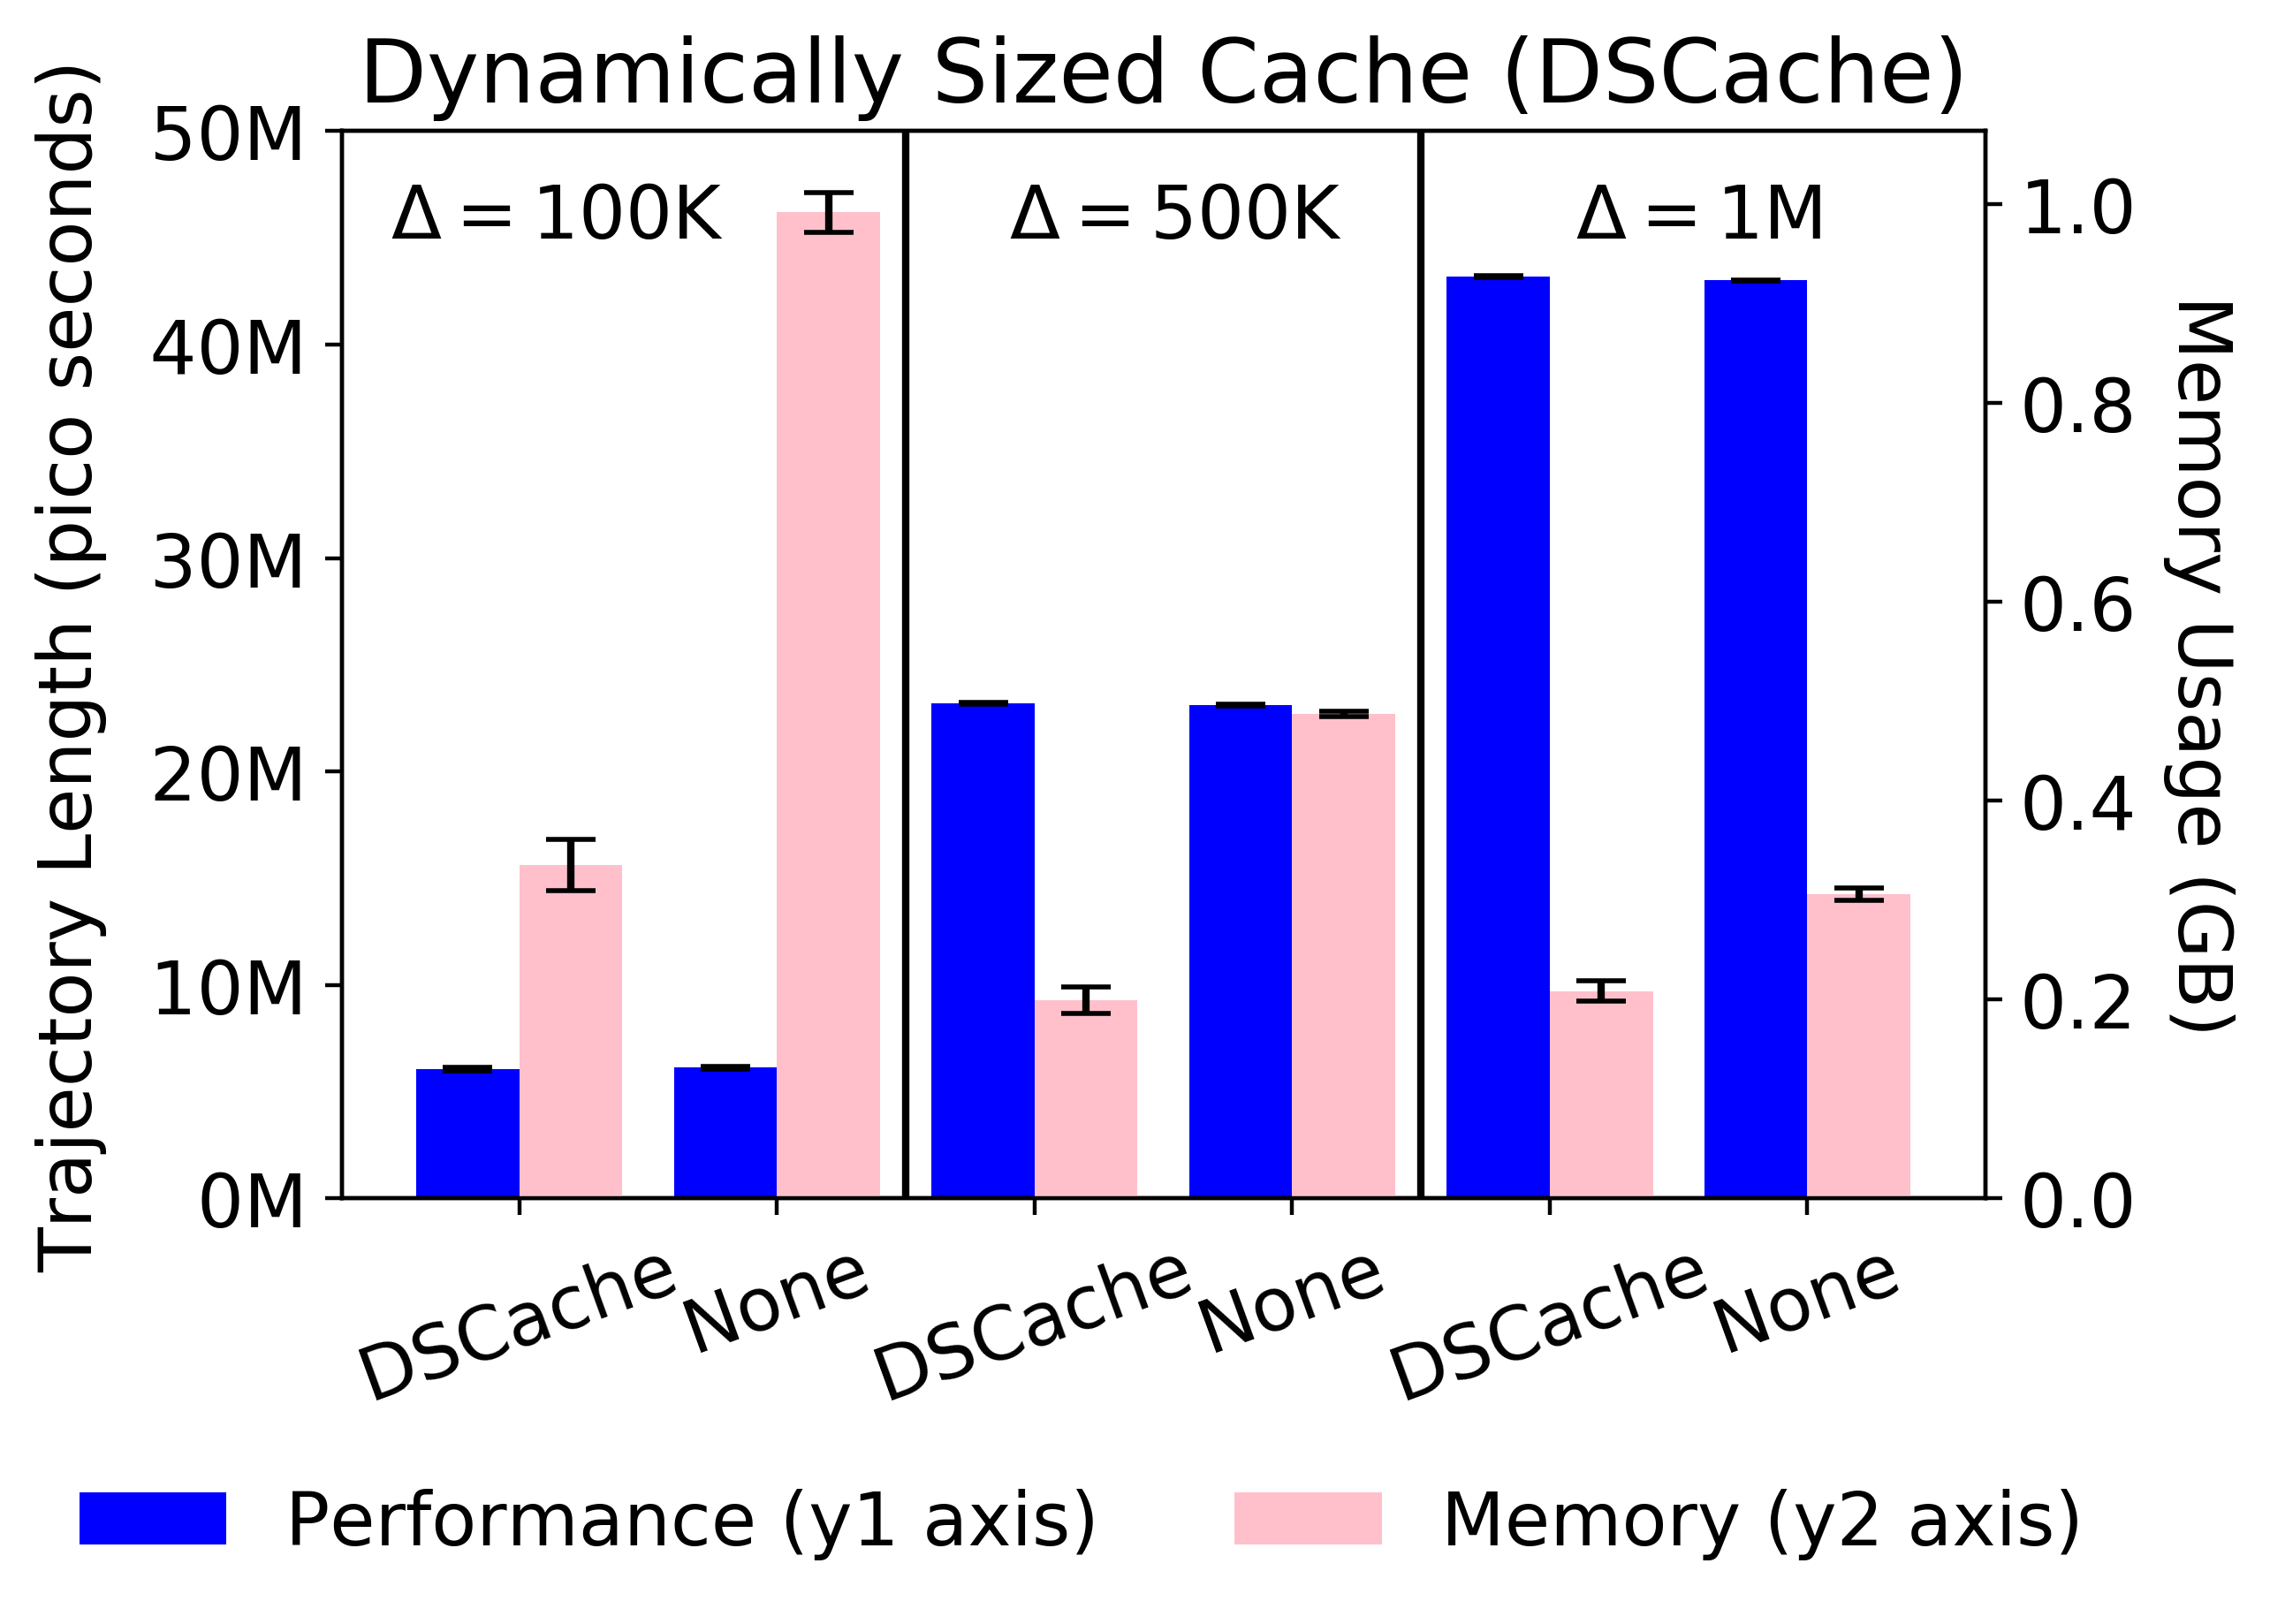
\includegraphics[width=1\textwidth]{./chapters/controlplane/parsplice/figures/dscache-vs-none.png}\\

	\caption{The performance/utilization for the dynamically sized cache (DSCache)
policy. With negligible performance degradation, DSCache adjusts to different initial configurations
(\(\Delta\)'s) and saves 3\(\times\) as much memory in the best case.
\label{fig:dscache-vs-none}}

    \end{subfigure}%
    \caption{Different cache management policies tested over the Mantle policy engine.}
\end{figure*}

\begin{figure}[tb]
\footnotesize
\begin{minted}[xleftmargin=3em,linenos]{lua}
d = timeseries()
ts, id = d:get(d:size())
fan  = {start=nil, finish=ts, top=0, bot=id}
fans = {}
for i=d:size(),1,-1 do     -- iterate backwards
  ts, id = d:get(i)
  if id < fan['bot'] then  -- found a new fan!
    fan['start']  = ts
    fans[#fans+1] = fan 
    fan = {start=nil, finish=ts, top=0, bot=id}
  end 

  if id > fan['top'] then  -- track top of fan
    fan['top'] = id 
  end 
end
fan['start'] = 0 
fans[#fans+1] = fan 

if #fans < 2 then -- do not evict current fan
  return false
else
  WRstate(fans[#fans-1]['top']-fans[1]['bot']) 
  return true
end
\end{minted}
\caption{The dynamically sized cache policy iterates backwards over
timestamp-key pairs and detects when accesses move on to a new subset of keys
({\it i.e.} ``fans"). The performance and total memory usage is in
Figure~\ref{fig:dscache-vs-none} and the memory usage over time is in
Figure~\ref{fig:memory-vs-time}.
\label{src:dyn-cache}}
\end{figure}

%\begin{figure}[t]
%  \noindent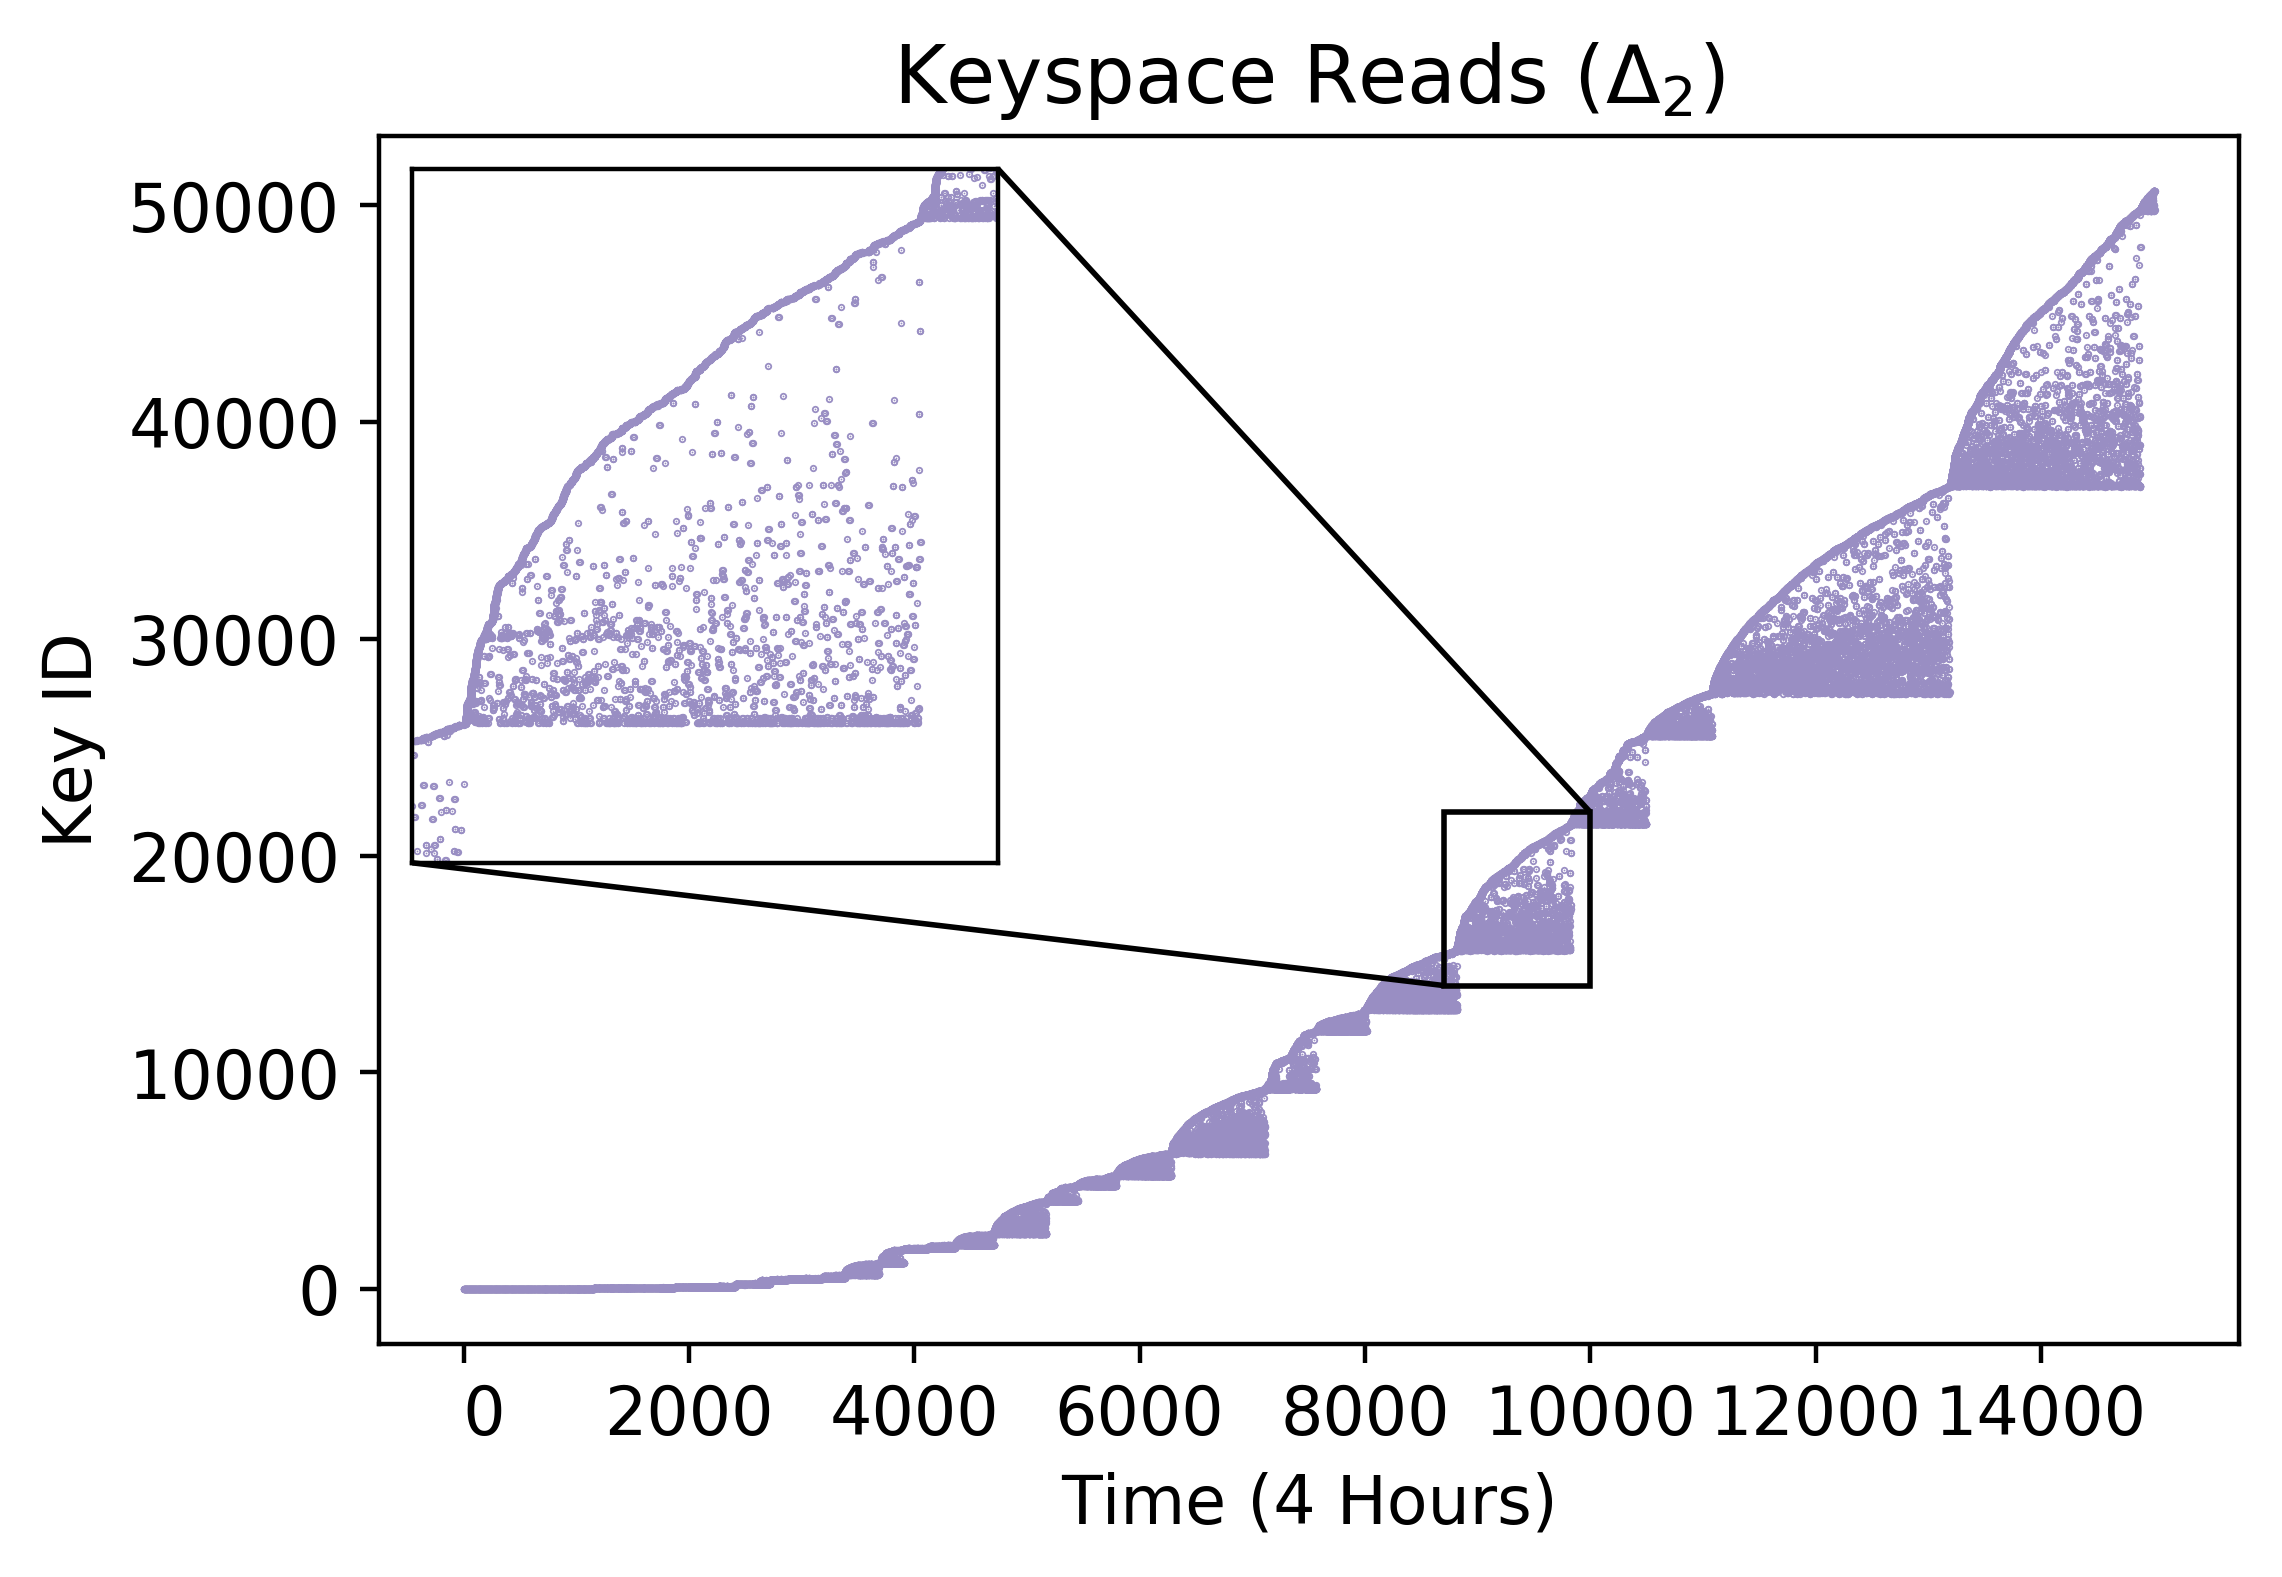
\includegraphics[height=5cm,width=0.4\textwidth]{./chapters/controlplane/parsplice/figures/keyspace-zoomed.png}\\
%
%  \caption{Key activity for a 4 hour run shows groups of accesses to the same
%  subset of keys. Detecting these access patterns leads to a more accurate cache
%  management strategy.\label{fig:keyspace-zoomed}}
%
%\end{figure}
%
%\begin{figure}[t]
%\noindent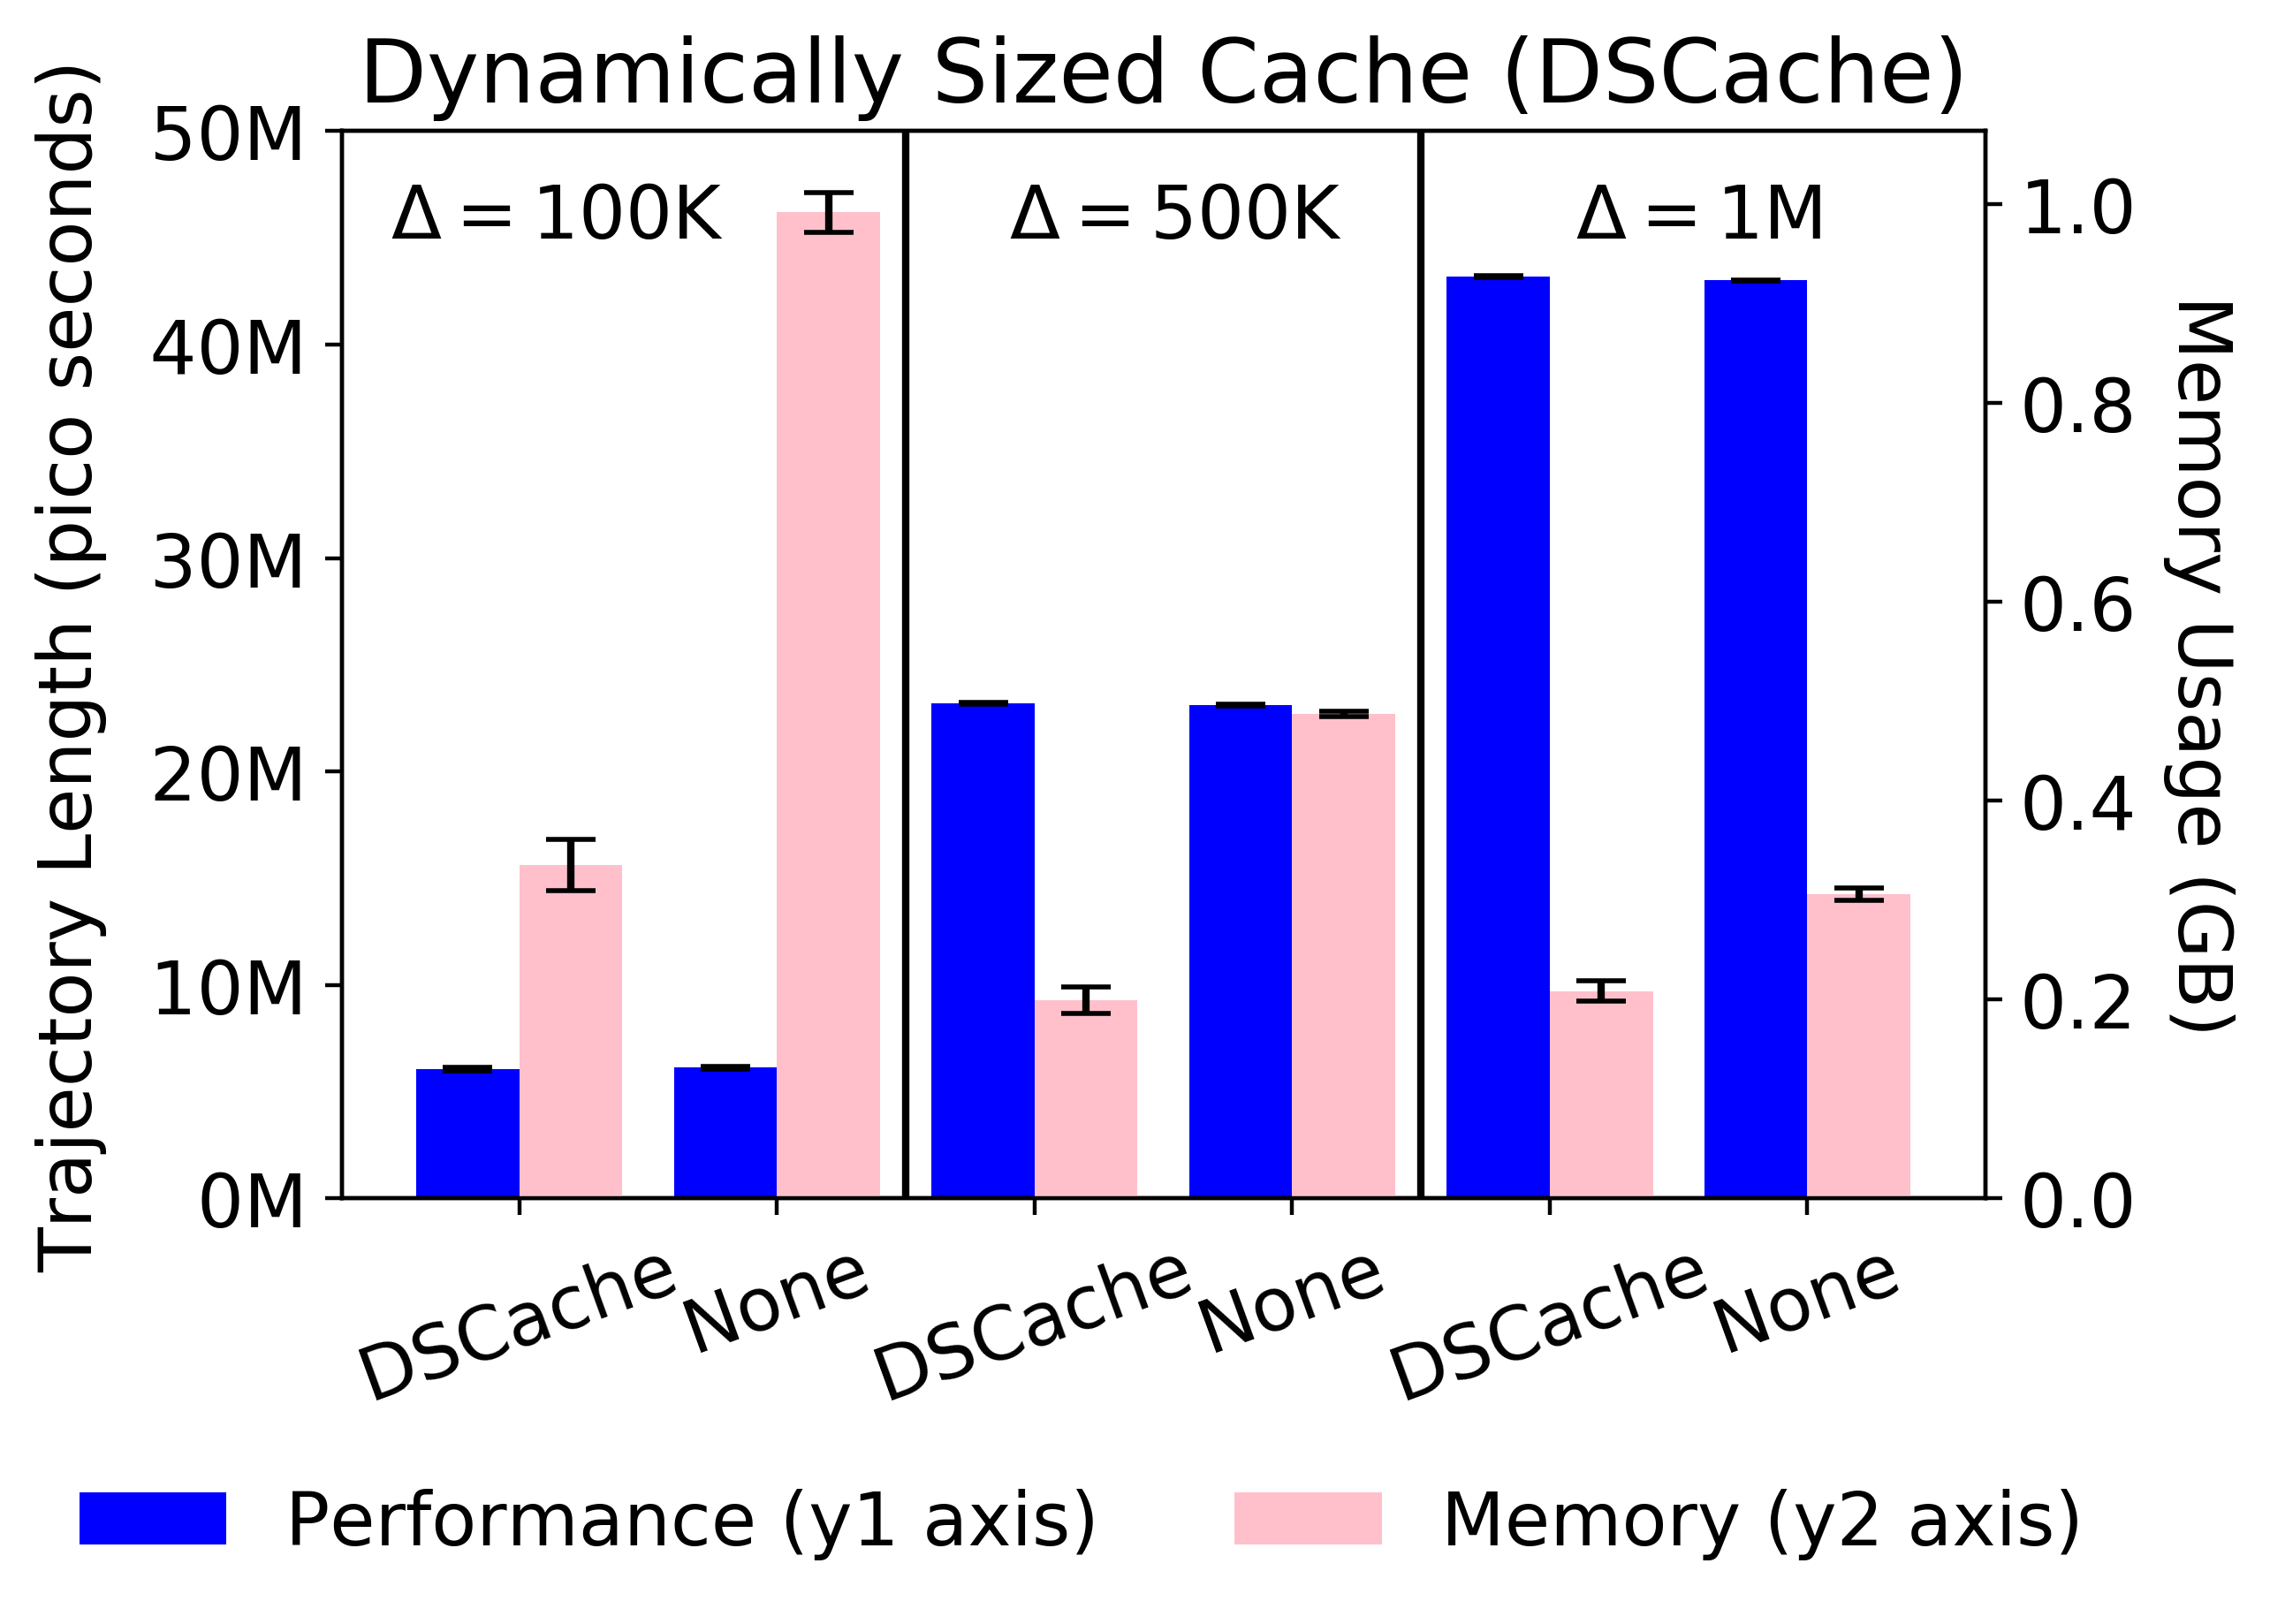
\includegraphics[width=0.5\textwidth]{./chapters/controlplane/parsplice/figures/dscache-vs-none.png}\\
%
%\caption{The performance and resource utilization trade-off for the dynamically
%sized cache (DSCache) policy compared to no cache management. With a negligible
%performance impact, DSCache adjusts to different initial conditions
%(\(\Delta\)) automatically and saves over 2\(\times\) memory in the best case.
%\label{fig:dscache-vs-none}}
%\end{figure}
%
%\begin{figure}[t]
%\noindent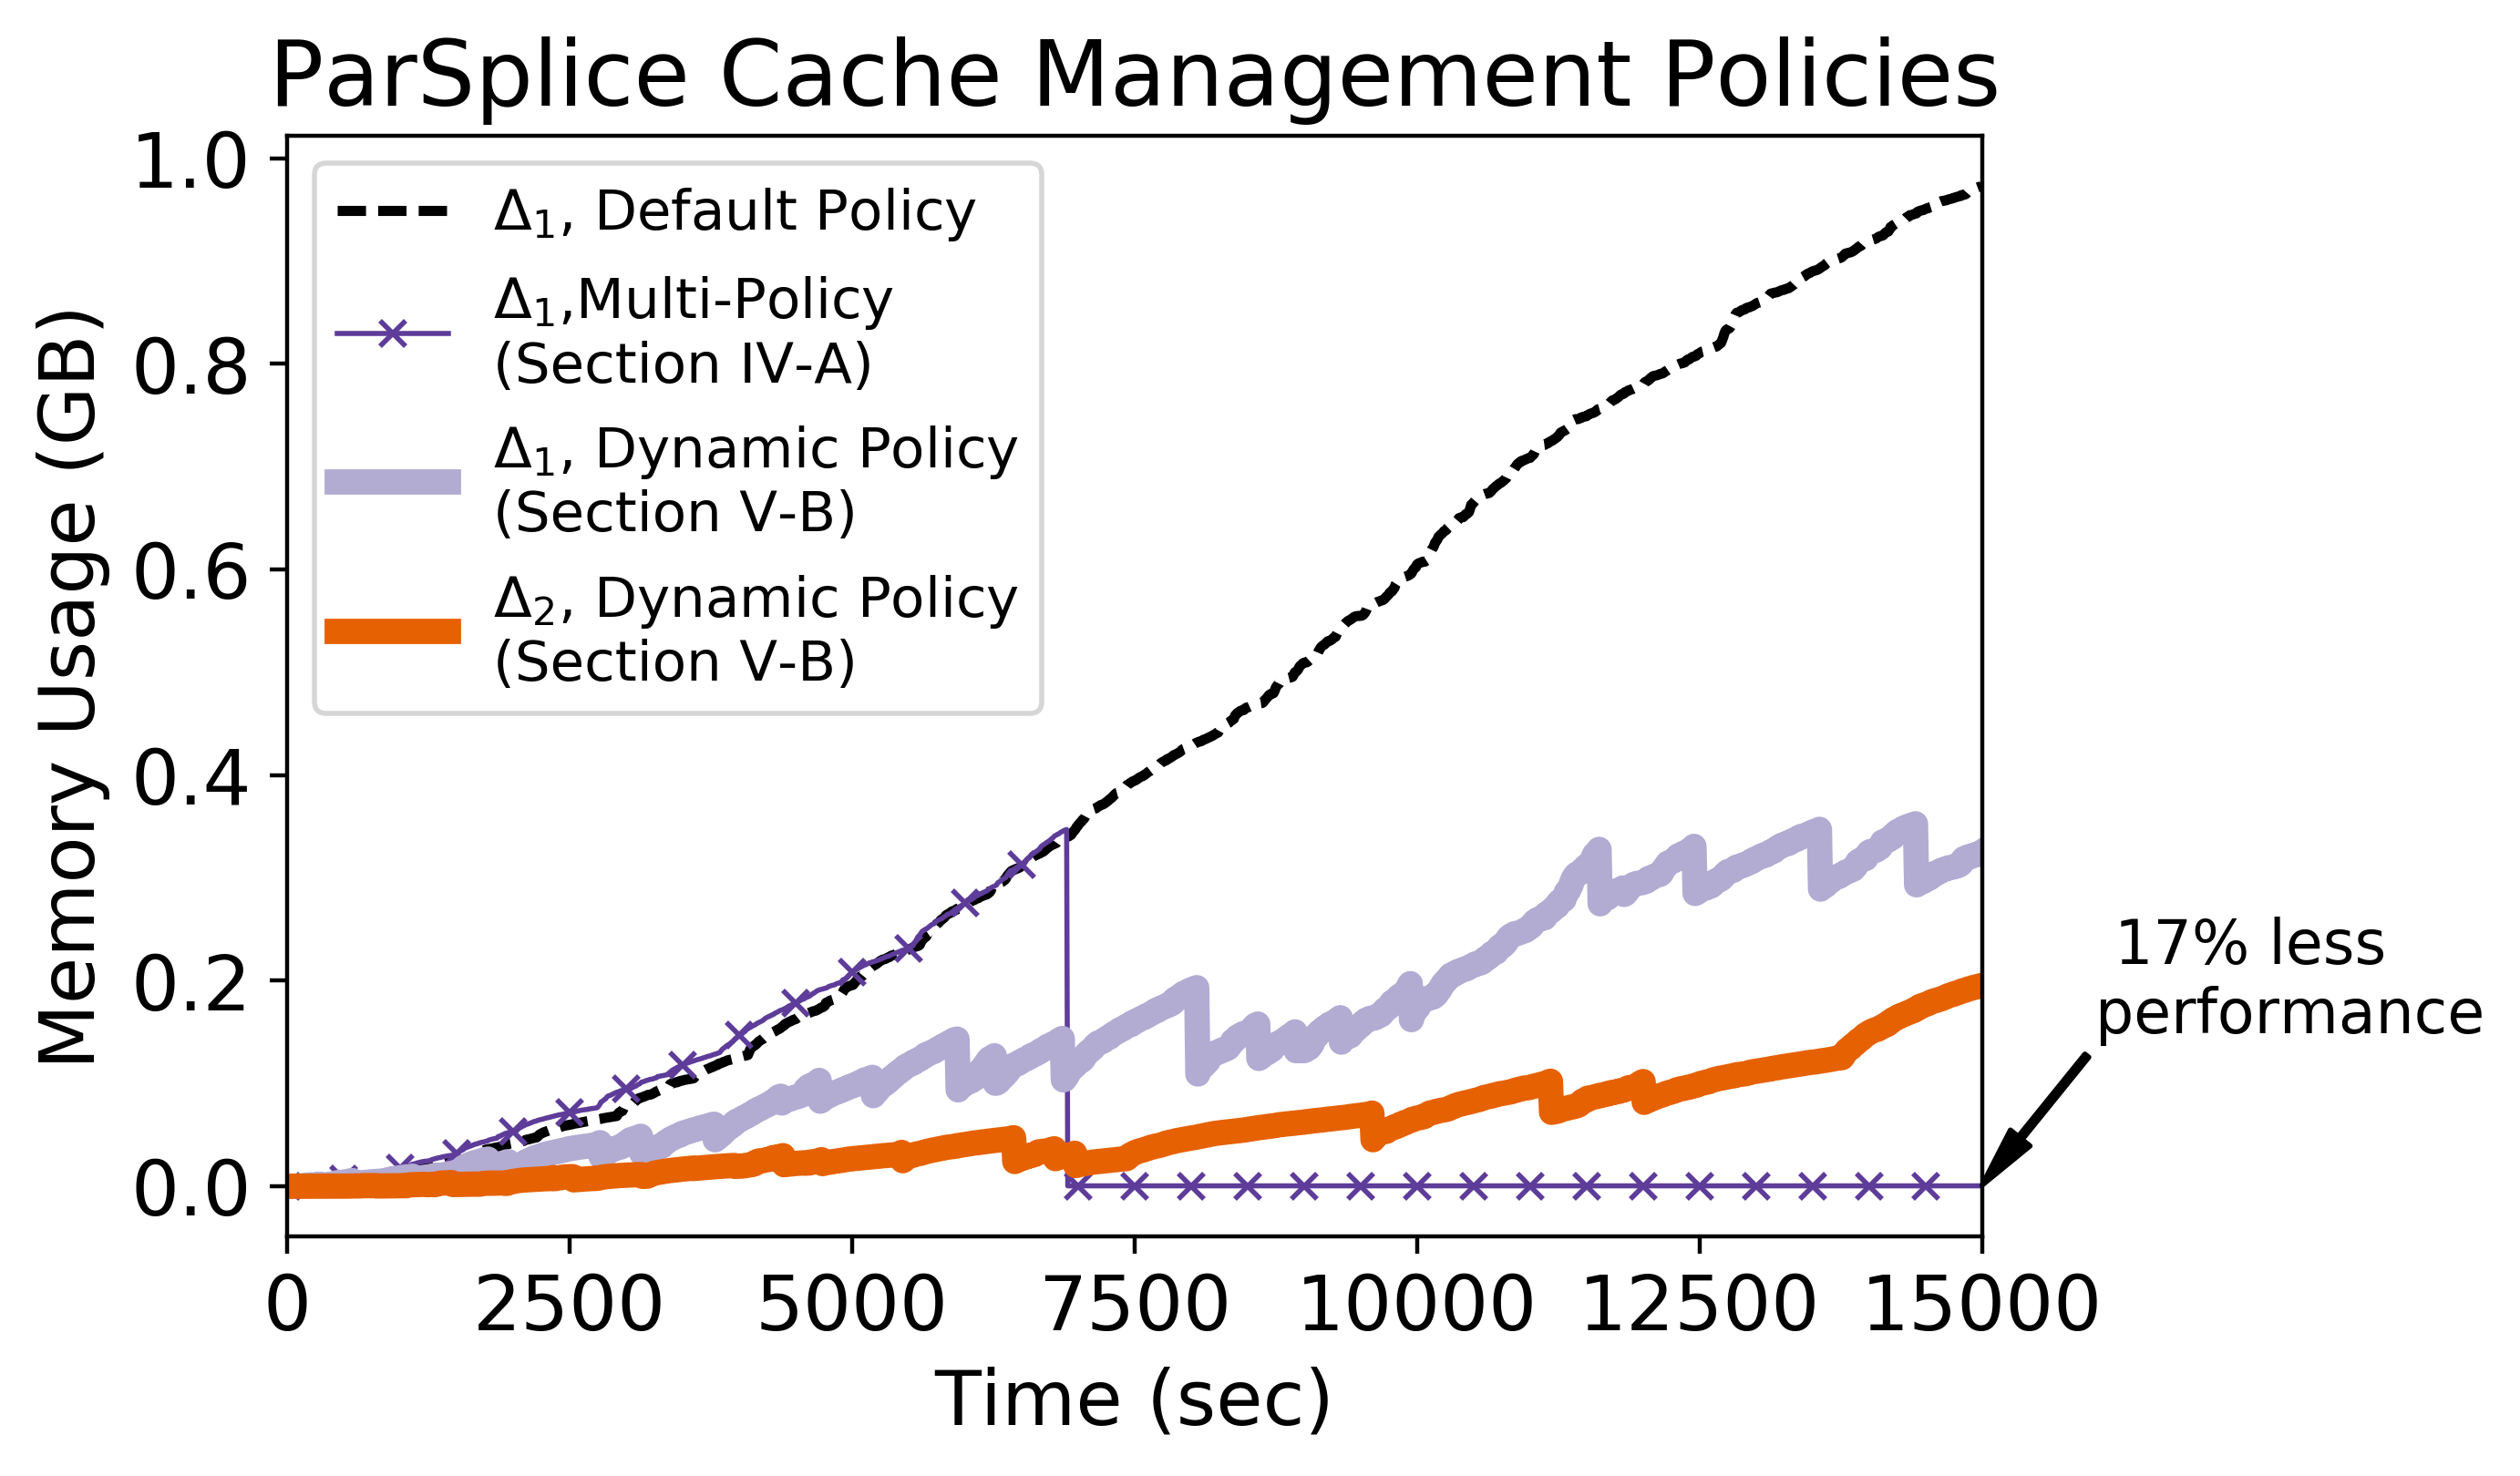
\includegraphics[width=0.5\textwidth]{./chapters/controlplane/parsplice/figures/memory-vs-time.png}\\
%
%\caption{Memory utilization of different cache management policies.  ``No Cache
%Management" allows unlimited cache growth, ``Multi-Policy" absorbs the initial
%burstiness of the workload before switching to a more constrained cache, and
%the ``Dynamic Policy" curves size the cache according to key access patterns.
%We show a \(\Delta_2\) growth rate to demonstrate the dynamic policy's ability
%to adjust to a different set of initial conditions.\label{fig:memory-vs-time}}
%\end{figure}

Feeding application-specific knowledge about ParSplice into a policy
leads to a more accurate cache management strategy.  The goal of the following
section is not to find an optimal solution, as this can be done with parameter
sweeps for thresholds; rather, we try to find techniques that work for a range
of inputs and system setups.

Figure~\ref{fig:keyspace-zoomed} shows which keys (\(y\) axis) are accessed by
tasks over time (\(x\) axis). The groups of accesses to a subset of keys occurs
because molecules are stuck in deep trajectories. Recall that the cache stores
the molecules' EOM minima, which is the smallest effective energy that a
molecule observes during its trajectory. So molecules stuck in deep
trajectories explore the same minima until they can escape to a new set of
states. This exploration of the same set of states is called a superbasin.  In
Figure~\ref{fig:keyspace-zoomed}, superbasins are never re-visited because the
simulation only adds molecules; we can never reach a state with less molecules.
This is why keys are never re-accessed.  

Detecting these superbasins can lead to more effective cache management
strategies because the height of the groups of key accesses is ``how much" of
the cache to evict and the width of the groups of key accesses is ``when" to
evict values from the cache.  The zoomed portion of
Figure~\ref{fig:keyspace-zoomed} shows how a single superbasin affects the key
accesses. Moving along the \(x\) axis shows that the number of unique keys
accessed over time grows while moving along the \(y\) axis shows that early
keys are accessed more often.  Despite these patterns, the following
characteristics of superbasins make them hard to detect:

\begin{itemize}

  \item superbasin key accesses are random and there is no threshold ``minimum distance
  between key access" that indicates we have moved on to a new superbasin

  \item superbasins change immediately

  \item the number of keys a superbasin accesses differs from other superbasins

\end{itemize}

\subsection{Failed Strategies}

To detect the access patterns in Figure~\ref{fig:keyspace-zoomed}, we try a
variety of techniques using Mantle. Unfortunately, we found that the following
techniques proliferate more parameters that need to be tuned per
hardware/software configuration. Furthermore, many of the metrics do not signal
a new set of key accesses.  Below, we indicate with quotes which parameters we
need to add for each technique and the value we find to work best, via
tuning and parameter sweeps, for one set of initial conditions.

\begin{itemize}

  \item Statistics: decay on each key counts down until 0; 0-valued keys are
evicted.  ``history-of-key-accesses", set to 10 seconds, to evict keys.

  \item Calculus: use derivative to strip away magnitudes; use large positive
slopes followed by large negative slope as signal for new set of key accesses.
``Zero-crossing", set to 40 seconds, for distance between small/large spikes to
avoid false positives; ``window size", set to 200 seconds, for the size of the
moving average.

  \item K-Means Clustering fails because ``K" is not known {\it a-priori} and
groups of key accesses are different size. ``K", set to 4, for the number of clusters in the data
using the sum of the distances to the centroid.

  \item DBScan: finds clusters using density as a metric. ``Eps", set to 20, for
max distance between 2 samples in same neighborhood; ``Min", set to 5, for the
samples per core.

  \item Edge Detection: size of the image is too big and bottom edges are
not thick enough.

\end{itemize}

\subsection{Dynamically Sized Cache: Access Pattern Detection}
\label{sec:regime-detection}

After trying these techniques we found that the basic O(\(n\)) algorithm in
Figure~\ref{src:dyn-cache} works best. The algorithm detects groups of key
accesses, which we call ``fans", by iterating backwards through the key access
trace, finding the lowest key ID, and comparing against the lowest key ID we
have seen so far (Line 7). We also maintain the top and bottom of each group of
key accesses (Line 13) so we can tell the ``how much" policy the number of keys
to evict (Line 23).  The algorithm is O(\(n\)), where \(n\) is the number
events, but the benefit is that the approach avoids adding new thresholds for
key access pattern detection ({\it e.g.}, space between key accesses, space
between key IDs, and window size of consecutive key accesses).

The algorithm iterates backwards over the key access trace because a change in
the minimum value signals a new group of key accesses. No signal exists
iterating left to right, as the maximum value always increases and the minimum
values at the bottom of each group of key accesses are sparse.  For example,
the maximum distance between values along the bottom edge of the zoomed group
of key accesses in Figure~\ref{fig:keyspace-zoomed} is 125 seconds, while the
maximum distance between minimum values for the group of key accesses before is
0 seconds. As a result of this sparseness, iterating left to right requires a
``window size" parameter to determine when we think a minimum value will not
show up again.  

The performance and memory utilization is shown by the ``DSCache" bars in
Figure~\ref{fig:dscache-vs-none}. Without sacrificing performance (trajectory
length), the dynamically sized cache policy uses between 32\%-66\% less memory
than the default ParSplice configuration (no cache management) for the 3
initial conditions we test. The memory usage over time is shown by the ``Dynamic Policy"
curves in Figure~\ref{fig:memory-vs-time}, where the behavior resembles the key
access patterns in Figure~\ref{fig:keyspace-zoomed}\footnote{The memory usage
is not {\it exactly} the same because these are two different runs;
Figure~\ref{fig:keyspace-zoomed} has key activity tracing turned on, which
reduces performance.}.  We also show a \(\Delta_2\) growth rate to demonstrate
the dynamic policy's ability to adjust to a different set of initial
conditions.


